\section{Gestor de Nodo}
El \textit{Node Management} es una entidad que se encuentra en el NMT, y es la
encargada de llevar a cabo el control de los nodos existentes en la red. En
esta entidad se encuentra almacenada la tabla de ruteo primario y secundario,
utilizado para lograr la correcta comunicación y configuración de la red.

El objetivo del gestor del nodo, es conocer todos los nodos que se encuentran
conectados en la red, y la distancia que existe entre el nodo actual y los
demás.

Por medio de las tablas de ruteo (primaria o secundaria en caso de fallas) el
nodo conoce a qué nodos puede enviar mensajes y a cuáles no. Debe aclararse que
nada impide enviar un mensaje a un nodo ``desconectado'', pero esta desición es
ineficiente y altamente peligrosa, ya que se puede estar enviando mensajes
críticos a un nodo ``caído''.

El gestor de nodo de cada dispositivo conectado a al red, es el encargado de
llevar a cabo el protocolo \textit{heartbeat}, el cual le indica a todos los
nodos conectados a la red que este está ``vivo''

En la Figura \ref{fig:Gestor_Nodo} se puede observar la arquitectura del Gestor
de Nodos.

\begin{figure}[h!]
 \centering
 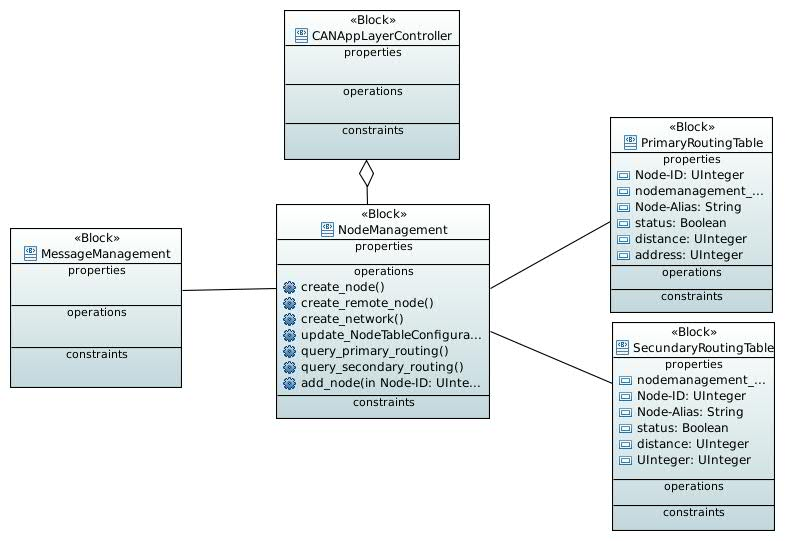
\includegraphics[scale=0.4]{images/Secciones/AppendixA/NodeManagement.JPG}
  \caption{Arquitectura del \textit{Node Management}}
\label{fig:Gestor_Nodo}
\end{figure}

\subsection{Tabla primara y secundaria de ruteo}\label{subsection:tablaprimariaysecundaria}
Los principales objetos del \textit{Node Management} son las tablas de ruteo.
Estas se las puede representar como una lista, en la cual se incluye
información de importancia para mantener actualizada la estructura de la red.
Los nodos se basarán sobre esta lista para tener conocimiento de los nodos
conectados a la red y con esto, llevar a cabo una correcta distribución de las
tareas.

Los algoritmos de ruteos se deben basar en estas tablas, ya que contienen toda
la información necesarias para cumplir con sus objetivos.

A continuación se detalla la tabla primara y tabla secundaria de ruteo.

\subsubsection{Tabla primaria}
La Tabla Primaria de Ruteo es la tabla principal estática utilizada por el
\textit{Node Management} para la gestión de los nodos de la red. Esta tabla
mantiene la a los n-iésimos nodos conectados a la red, desde el punto de vista
del nodo ``actual''. Es decir, para cada nodo existe una y sola una tabla, y esa
tabla es única en la red, ya que es creada desde el punto de vista del nodo
``host''.

La estructura de la lista es simple. Cada renglón de la lista es un nodo, siendo
el primer renglón obligatoriamente el nodo de la tabla, llamado nodo ``host''.
Los siguientes renglones de la lista representan los demás nodos conectados a la
red. Por convención, los nodos se listan comenzando por los vecinos de derecha a
izquieda. Luego se continúa la lista tratando de seguir la convención de derecha
a izquierda.

La tabla tiene la siguiente estructura:
\begin{itemize}
\item \textbf{UIntegerNode-ID}: Es el ID único para cada nodo. 
\item \textbf{String Node-Alias}: Es el alias para cada nodo. Este alias puede
  ser utilizado para comodidad por parte del usuario para referenciar los nodos.
\item \textbf{UInteger Address}: Es la dirección del nodo.  
\item \textbf{Boolean Status}: Es el estado del nodo. Pude ser \{ CONNECTED,
  DISCONNECTED \}.
\item \textbf{UInteger Distance}: Es la distancia (cantidad de nodos) que hay
  entre el nodo  ``host'' y los demás nodos de la red. 
\end{itemize}

\subsubsection{Tabla secundaria}
La Tabla Secundaria de Ruteo es una tabla estática similar que la Tabla Primara
de Ruteo, con la diferencia sustancial que es utilizada cuando hay fallas en el 
ruteo. Esta tabla se genera cuando se producen fallas en uno o más nodos, y se
necesita conocer la estructura de la red, para luego tomar desiciones sobre la
configuración de la misma.

La estructura de la Tabla Secundaria de Ruteo es similar a la Tabla Primara de
Ruteo. La diferencia sutancial es que no se encuentran todos los nodos de la
red, sino aquellos que se encuentran ``funcionales''.

La estructura de la tabla se detalla a continuación:
\begin{itemize}
\item \textbf{UIntegerNode-ID}: Es el ID único para cada nodo. 
\item \textbf{String Node-Alias}: Es el alias para cada nodo. Este alias puede
  ser utilizado para comodidad por parte del usuario para referenciar los nodos.
\item \textbf{UInteger Address}: Es la dirección del nodo.
\item \textbf{Boolean Status}: Es el estado del nodo. Pude ser \{ CONNECTED,
  DISCONNECTED \}.
\item \textbf{UInteger Distance}: Es la distancia (cantidad de nodos) que hay
  entre el nodo  ``host'' y los demás nodos de la red. 
\end{itemize}

\subsection{Servicios}
Los servicios brindados por el \textit{Node Management} son los siguientes:
\begin{itemize}
\item Boolean create\_node(UInteger Node-ID, UInteger address, String
  description): esta función crear el objeto nodo. Este servicio ya fue
  descripto en \ref{subsubsection_servicios_implementar}. Entre otras cosas,
  este servicio crea la primera entrada en la Tabla Primaria de Ruteo. 
  \begin{itemize}
  \item \textbf{UInteger Node-ID}: ID del nodo a crear.
  \item \textbf{UInteger address}: Dirección del nodo creado. UInteger entre [0,255]
  \item \textbf{String description}: Descripción del nodo.
  \end{itemize}

\item Boolean connect\_remote\_node(UInteger Node-ID): envía la señal a sus
  nodos vecinos para que creen una referencia de este nodo en los demás. 
  \begin{itemize}
    \item \textbf{UInteger Node-ID}: ID del nodo remoto a conectar.
  \end{itemize}

\item Boolean create\_network(): esta función fue descrita en
  \ref{subsubsection_servicios_implementar}. Este servicio crea una instancia de
  la Tabla Primara de Ruteo.

\item Boolean update\_NodeTableConfiguration(): esta función actualiza la tabla
  de configuración del nodo
  (Vista en: \ref{subsubsection_servicios_implementar}).

\item Data query\_primary\_routing(): esta función lleva a cabo una consulta a
  la Tabla Primaria de Ruteo. Se la utiliza cuando se necesita extraer datos de
  la configuración de la red.

\item Data query\_secundary\_routing(): esta función lleva a cabo una consulta a
  la Tabla Secundaria de Ruteo. Se la utiliza cuando se necesita extraer datos de
  la configuración de la red luego de fallas en los nodos.

\item Boolean add\_node(UInteger Node-ID, String Node-Alias, Boolean status,
  UInteger distance, UInteger address): este servicio se lleva a cabo cuando
  llega el mensaje connect\_remote\_node(UInteger Node-ID). Este servicio
  agrega un node (renglón) en la Tabla Primaria de Ruteo.
  \begin{itemize}
  \item \textbf{UInteger Node-ID}: ID del nodo a agregar.
  \item \textbf{String Node-Alias}: Alias del nodo a agregar.
  \item \textbf{Boolean status}: Estado del nodo. CONNECTED=1, DISCONNECTED=0.
    Por defecto los nodos están en estado 1 (CONNECTED).
  \item \textbf{UInteger distance}: Distancia que existe entre el nodo
    ``host'' y el nodo a agregar.
  \item \textbf{UInteger address}: Dirección del nodo a agregar.
  \end{itemize}     
\end{itemize}



